%% ------------------------------------------------------------------------- %%
\chapter{Conceitos}
\label{cap:conceitos}


\section{Definição do Problema}


Os dados da Intercement são anotados temporalmente, então podemos escolher
trata-los como uma série temporal, i.e. a ordem de entrada dos dados no modelo
importa. A tarefa de regressão se torna então prever próximas anotações desses
dados num horizonte de tempo futuro finito. O problema é de Aprendizado
Supervisionado, buscamos a distribuição das anotações $y$ condicionada
aos parâmetros de entrada $x$, mas também ao
histórico da série temporal, i.e. valores passados do objetivo $y$. A série
temporal é composta por diversas medições indexadas pelo tempo $t$ do objetivo
de predição $y$ e de um vetor $\textbf{x}$ de parâmetros independentes.


Seja um série temporal alvo, $Y$, e diversas séries temporais de variáveis
independentes $X_i$ com entradas nas anotações de tempo no intervalo $[1,T]$. Seja $T$ o último dia em que se possui dados de ambas essas
séries. Desejamos modelar a distribuição de probabilidade das próximas anotações
de $Y$ até da nova data $F + T$, $F \in \mathbb{N}$, condicionadas por uma janela de
observações das diversas variáveis independentes $X_i$ e do alvo $Y$ no passado.

\[ p(y_{T:F} | y_{1:T},\textbf{x}_{{1}:T}) \]

A distribuição será aprendida por meio de aprendizado supervisionado, onde os
modelos serão alimentados com diversos pares de entradas,
$(y_t,\textbf{x}_{(t-W):t})$, onde $\textbf{x}$ é um vetor contendo os valores de
cada variável independente $X_i$, no instante de tempo $t$. Cada tupla de
entrada contém $W$ entradas do vetor de variáveis independentes. O parâmetro $W$, o
tamanho da janela de tempo consumida para gerar cada saída, é escolhido antes do
treino e pode ser alterado na busca de uma melhor acurácia de predição.

\section{Estatística Frequentista e Estatística Bayesiana}
 
Como nesse trabalho serão usados métodos de inferência Bayesiana aplicados a ML,
cabe então uma breve elaboração das diferenças entre as duas principais
vertentes da estatística. O seguinte desenvolvimento é retirado de \citep{dlbook}:\\

Digamos que exista um evento aleatório que tenha um resultado com probabilidade
$p$ de acontecer. A visão frequentista de probabilidades diz que, se pudéssemos repetir infinitas vezes esse evento, a proporção de vezes que esse resultado irá acontecer se aproximará arbitrariamente de $p$. E então entenderíamos a probabilidade $p$ meramente como uma proporção de resultados positivos em uma certa amostra de experimentos. Mas e se o evento não pudesse ser repetido? Quando físicos criam modelos para explicar o nascimento do universo, é impossível pensar em repetir o Big Bang infinitas vezes para que se possam estimar probabilidades de certos eventos cosmológicos acontecerem. Nesse segundo caso, resultados são derivados de \textbf{graus de certeza}, onde a chance de um evento acontecer é estimada pela aplicação de conhecimentos prévios em vista de algo que foi observado posteriormente. A primeira maneira de se entender estatística é chamada de Frequentista e a segunda de Bayesiana. \\

E no campo de ML, as duas maneiras de se gerar predições são estimadores
frequentistas (Seção~\ref{sec:est}) e inferência Bayesiana (seção~\ref{sec:bayesinf}).



\section{Aprendizado Automático}

O campo de Aprendizado Automático (Machine Learning - ML) é um ramo da Ciência
da Computação que utiliza métodos estatísticos para criar sistemas que possam
aprender a realizar uma determinada tarefa através de dados. Um problema de ML possui
as seguintes partes \citep{dlbook}: \\

\begin{itemize}

  
\item A tarefa $T$, no caso dos dados da Intercement, um problema de regressão.
  Onde desejamos estimar valores numéricos a partir de uma matriz de dados $X$ e
  suas anotações numéricas $Y$. 
  
\item Uma métrica de performance $P$, que define a distância entre as predições
  do modelo e os dados de treinamento. A teoria por trás desses métricas será explicada na seção~\ref{sec:metricas}.

\item A experiência $E$, que define qual tipo de informação o modelo poderá usar
  durante o treinamento. Explicaremos esse conceito na seção~\ref{sec:exp} 
  
\end{itemize}

\subsection{A Experiência}
\label{sec:exp}
Algoritmos de ML podem ser divididos nas categorias de aprendizado supervisionado, não supervisionado e aprendizado por reforço \citep{dlbook}. Técnicas dos dois primeiros tipos serão usadas para os dados da Intercement.


\subsubsection{Aprendizado Supervisionado}
\label{sec:apren} 
Aprendizado Supervisionado consiste, do ponto de vista estatístico, em aprender uma distribuição
de probabilidade condicional do tipo $p(y | x)$. Nos são fornecidos diversos vetores de
entrada $x$ associados a uma anotação $y$ e gostaríamos de modelar essa relação
entre dados e anotações para que possamos anotar novos dados inéditos para os
modelos. Ou seja, para diversos exemplos de vetores
$x$ são fornecidas anotações $y$, e desejamos então criar predições de anotações
$y'$ para novas entradas $x'$.


\subsubsection{Aprendizado Não Supervisionado}

Para o caso de Aprendizado Não Supervisionado, mantendo a estrutura do exemplo
anterior, desejaríamos então modelar uma distribuição do tipo $p(x)$, onde temos
também diversos exemplos de vetores aleatórios $x$ e estamos estudando alguma propriedade importante dessa distribuição.



\subsection{A Performance}
\label{sec:metricas}

\subsubsection{Estimadores}
\label{sec:est}

A aprendizagem estatística busca a diminuição de \textit{risco} das predições feitas por
um modelo \citep{mlprob}.

Um método usual da diminuição de risco é a de buscar guiar o aprendizado pela
maximização da verossimilhança do modelo. Esse valor é a probabilidade de termos
observado os dados alvo condicionada pelos parâmetros do modelo e as entradas
(que iremos representar pelo vetor $\theta$). Uma iteração de
treino então consistira do produtório de todas as verossimilhanças para cada par
de entradas. Generalizando essa ideia, na definição do nosso problema, temos que o custo total do modelo
$\mathcal{L}$ é dado por:

\[
\mathcal{L} = \prod_{t=W}^{i=T} p(y_t=\hat{y_t} | \textbf{x}_{(t-W):t}, \theta) 
\]

É comum, porém, por motivos de estabilidade numérica \citep{dlbook}, substituir
o produtório de probabilidades pelo somatório do logarítimo das probabilidades: 

Para modelos com baixa dimensionalidade e muitos dados, a estimativa bayesiana
coincide com a frequentista, convergindo para a \textbf{estimação de máxima
verossimilhança} \citep{mlprob}. Isso se deve ao fato que a distribuição de
probabilidade a priori progressivamente se torna menos importante no calculo da
probabilidade posterior com muitos dados.


\[
  \mathcal{L} = \sum_{t=W}^{i=T} \log{p(y_t=\hat{y_t} | \textbf{x}_{(t-W):t},\theta)}
\]


Na seção~\ref{sec:reglog} iremos dar um exemplo dessa cálculo de verossimilhança
assumindo que o erro do modelo é distribuído normalmente.

\subsubsection{A Distribuicão Normal}
\label{sec:reglog}

Uma variável aleatória Y distribuida normalmente possui uma funcão densidade de
probabilidade da seguinte forma \citep{mlprob}:

\begin{equation}
  \label{eq:ver}
p(y| \mu,\sigma^2) = \frac{1}{\sqrt{2\pi\sigma^2}}\exp{-\frac{(y - \mu)^2}{2\sigma^2}}
\end{equation}

Esse valor também é chamado de verossimilhança (a probabilidade de termos
observado um valor de Y, dado que essa variável é distribuída normalmente, com média $\mu$ e variância $\sigma^2$), e
normalmente trabalha-se com o logarítimo desse valor, para podermos trocar um
produtório por somatório para agregar os erros gaussianos de um conjunto de dados
i.i.d.. Nesse caso, temos pares de predição e valor real, que assumirá o papel
da média $\mu$. A verossimilhança total de um conjunto de diversos pares
$(\hat{y},y)$ é dado por: 

\begin{equation}
\label{eq:logver1}
  \mathcal{L}= -m \log \sigma - \frac{m}{2} \log (2 \pi) - \sum^m_{i=1}
  \frac{\abs{\hat{y_i}-y_i}^2}{2 \sigma^2}
\end{equation}

Um estimador sem viés da Equação~\ref{eq:logver1}, chamado de Erro Quadrático
Médio, pode ser escrito apenas como \citep{mlprob}:

\begin{equation}
  \label{eq:logver2}
  \mathcal{L}=  \sum^m_{i=1} (\hat{y_i}-y_i)^2
\end{equation}


\subsubsection{Função de Custo}

A Função de Custo, derivada diretamente da verossimilhança,
é uma função usada para guiar os algoritmos de otimização na direção de parâmetros que melhorem a performance do modelo \citep{dlbook}. Isso é feito, como explicado na Sessão~\ref{sec:reglog}, aproximando a distribuição gerada pelo modelo da distribuição observada pelos dados. \\

Nessa sessão iremos definir a função de custo usada em todos os modelos de regressão usados. \\

\subsubsection{Erro Quadrático Médio}
\label{sec:MSE}

O Erro Quadrático Médio é um estimador não enviesado da Equação~\ref{eq:ver}
\citep{dlbook}. Ele é calculado em relação a duas variáveis contínuas
$(\hat{y},y)$, definido da seguinte forma:

\[MSE = \sum^n_{i=1}\frac{(\hat{y_i} - y_i)^2}{n}\]

Essa métrica é uma medida absoluta. E quanto maior esse valor pior o desempenho
do modelo, i.e. mais distante suas predições estão da média real. \\

\subsubsection{Divergência KL}

A divergência KL, ou Kullback-Leibler, é uma medida de diferença entre duas distribuições de probabilidade (também chamada de Entropia Relativa). \\
Essa medida pode ser definida pelo valor esperado da diferença logarítmica da probabilidade dos dados serem observados em uma distribuição ou na outra \citep{dlbook}. \\
Sejam duas distribuições de probabilidade $p$ e $q$, bem como uma matriz de dados $X$: \\

\[D_{KL}(p || q) = \mathop{\mathbb{E}}[\log p(x) - \log q(x)]​\]

Ou em uma forma mais usual: \\

\[D_{KL}(p||q) = \sum_{i=1}^{N}p(x_{i}) \log \frac{p(x_{i})}{q(x_{i})}​\]



\subsection{Métrica de Acurácia}

Diferentemente da função de custo, a métrica de acurácia não é usada para guiar a otimização do modelo,
mas para testar as predições frente a realidade e avaliar sua qualidade. \\

\subsubsection{R-quadrado}
Como teste da acurácia dos modelos foi usada a métrica R-quadrado ($R^2$) \citep{cohen}. Sejam $\hat{y}$ e $y$ nossa previsão dada pelo modelo e o seu valor real, a acurácia do modelo é dada por:\\

\begin{align}
&R^2 = 1 - \frac{SS_{res}}{SS_{tot}} &\\
&SS_{tot} = \sum^n_{i=1} (y_i- \hat{y_i})^2 &\\
&SS_{res} = \sum^n_{i=1} (y_i - \bar{y})^2 &\\
&\bar{y} = \frac{1}{n} \sum^n_{i=1} y &
\end{align}

% \justify
$SS_{res}$ mensura a quantidade de variância \textit{residual}, a
variância entre os dados reais e as predições do modelo, i.e. a variância não
explicada pelo modelo. $SS_{tot}$ cumpre o papel da variância \textit{total}. A métrica $R^2$
então nos mostra quanto da variância dos dados é explicada pelo modelo. \\

Para essa métrica, o modelo pode ter um desempenho arbitrariamente ruim, com esse valor
podendo se tornar arbitrariamente negativo. Porém, seu valor máximo é 1,
indicando um modelo ideal.\\


\subsubsection{Custo quantílico}

O custo quantílico é usado na avaliação de performance de predições temporais. \\
Dado um quantil $p \in (0,1)$ um valor real $y_{t}$ e uma predição $y^{*}_{t}(\rho)$, esse valor é definido por: \\

\begin{equation}
  \mathcal{QL}_{\rho}(y_{t},y^{*}_{t}(\rho)) =
\begin{cases*}
  2 \rho(y_{t} - y^{*}_{t}(\rho)) & se $ y_{t} - y^{*}_{t}(\rho) > 0$ \\
  2 (1 - \rho)(y^{*}_{t}(\rho) - y_{t}) & se $y_{t} - y^{*}_{t}(\rho) \leq 0$
\end{cases*}
\end{equation}


%% ------------------------------------------------------------------------- %%


\section{Modelos Clássicos} 



\subsection{Regressão Linear}

Um modelo de Regressão Linear é da forma \citep{bayesml}:
\begin{equation}
 \label{eq:linreg}
  p(y| x, \theta) = \mathcal{N}(y | \omega^\intercal x, \sigma^2)
\end{equation}

O vetor $\omega$ é aprendido por meio do métodos dos mínimos quadrados, que é
uma maximização da verossimilhança da Equação~\ref{eq:linreg}.


\subsection{Redes Neurais}

\label{sec:nn}
Redes neurais são aproximadores universais de funções \citep{nnuni}. Dado um problema
de classificação onde se deseja aprender uma função da forma $y = f^*(x)$, uma
Rede Neural define um mapeamento $y = f(x ; \theta)$, onde $\theta$ é o vetor de
parâmetros que serão aprendidos com o fim de minimizar a diferença entre a
distribuição empírica e essa distribuição gerada pelo modelo. Essa diferença pode
ser minimizada pelo método da verossimilhança, assim como elaborado na sessão~\ref{sec:reglog}.\\

O modelo neural é uma composição de funções que unem uma transformação linear e
a aplicação de uma função não-linear $\sigma$: \\

\[ f(x)=  \sigma(W*x + b) \]

Importante ressaltar que $W$ é uma matriz, assim como $x$ e $b$ são vetores. \\

Auma  computação da saída de uma rede neural então pode ser escrita como:

\[   y = f_n \circ f_{n-1} \circ f_{n-2} \dots f_1(x)  \]

Para uma rede neural de $n$ \textbf{camadas}, onde cada camada será uma função
$f_i$ cujos parâmetros são $W_i$ e $b_i$. Portanto, para a i-ésima camada da rede
sua saída será da forma: 

\[ f_i (x)=  a_i = \sigma(W_i*a_{i-1} + b_i) \]

Onde $a_{i-1}$ é a saída da camada anterior, também chamada de
\textbf{ativação}. A saída dessa camada é então a sua ativação $a_i$. \\ 

Vale notar que uma saída $y$ calculada por uma rede neural depende unicamente dos
seus parâmetros e da entrada $x$. Isso não será verdade para os modelos
\textbf{sequenciais} que também serão usados nesse trabalho, onde o estado
interno de computação desses modelos é usado como entrada para uma próxima
iteração \citep{dlbook}. \\

Na Figura~\ref{fig:nn} mostramos como seria uma rede que usa os índices RC3 e RC7 para
modelar como saída o índice RC28. \\  

\begin{figure}
  \centering
  \def\layersep{2.5cm}

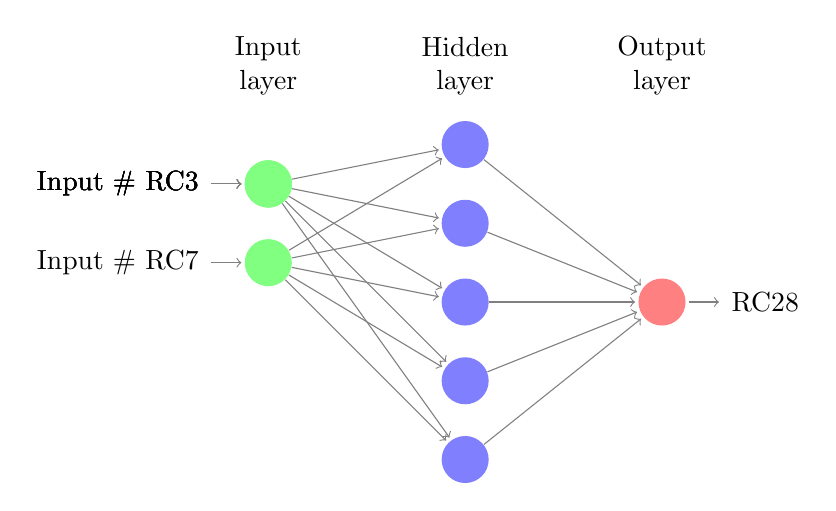
\begin{tikzpicture}[shorten >=1pt,->,draw=black!50, node distance=\layersep]
    \tikzstyle{every pin edge}=[<-,shorten <=1pt]
    \tikzstyle{neuron}=[circle,fill=black!25,minimum size=17pt,inner sep=0pt]
    \tikzstyle{input neuron}=[neuron, fill=green!50];
    \tikzstyle{output neuron}=[neuron, fill=red!50];
    \tikzstyle{hidden neuron}=[neuron, fill=blue!50];
    \tikzstyle{annot} = [text width=4em, text centered]

    % Draw the input layer nodes
    \foreach \name / \y in {1,...,4}
    % This is the same as writing \foreach \name / \y in {1/1,2/2,3/3,4/4}
    \node[input neuron, pin=left:Input \# RC3] (I-1) at (0,-1) {};
    \node[input neuron, pin=left:Input \# RC7] (I-2) at (0,-2) {};

    % Draw the hidden layer nodes
    \foreach \name / \y in {1,...,5}
        \path[yshift=0.5cm]
            node[hidden neuron] (H-\name) at (\layersep,-\y cm) {};

    % Draw the output layer node
    \node[output neuron,pin={[pin edge={->}]right:RC28}, right of=H-3] (O) {};

    % Connect every node in the input layer with every node in the
    % hidden layer.
    \foreach \source in {1,...,2}
        \foreach \dest in {1,...,5}
            \path (I-\source) edge (H-\dest);

    % Connect every node in the hidden layer with the output layer
    \foreach \source in {1,...,5}
        \path (H-\source) edge (O);

    % Annotate the layers
    \node[annot,above of=H-1, node distance=1cm] (hl) {Hidden layer};
    \node[annot,left of=hl] {Input layer};
    \node[annot,right of=hl] {Output layer};
\end{tikzpicture}
  \caption{Um exemplo de Rede Neural no contexto dos dados da Intercement}
  \label{fig:nn}
\end{figure}


\bigskip

 
\subsection{Random Forest}

Random Forests são um método de \textbf{Ensemble Learning} para classificação ou regressão. \textbf{Ensemble Learning} é uma família de técnicas no qual diversos modelos "fracos" são usados em conjunto com algum sistema de votação para que a a acurácia do sistema em conjunto se torne melhor que a de qualquer um dos modelos sozinho. Seguindo essa ideia, Random Forests são conjuntos de diversas árvores de decisão simples unidas por um meta-algoritmo de votação para que se produza uma predição muito mais eficaz.


\section{Modelos Sequenciais}
Com o sucesso de modelos sequenciais no campo do Deep Learning, iremos averiguar se é possível modelar sequencialmente os dados da produção de cimento usando dois desses modelos. 

\subsection{Rede Neural Recorrente}
% 
\scalebox{1}{
\begin{tikzpicture}[auto]

% RNN state cell =============================
\node[state] (h) {$\vect{h}$};
\node[op, below=30pt of h] (x) {$\vect{x}$};
\node[op, above=30pt of h] (yhat) {$\hat{\vect{y}}$};



% edges
\path[tedge] (x) edge node[below right= -4pt] {$\vect{U}$}  (h) ;
\path[tedge] (h) edge [out=-400,in=-320,looseness=8, distance=125pt] node[above right] {$\vect{W}$} (h);
\path[tedge] (h) edge node[below right = -4pt] {$\vect{V}$} (yhat);


\end{tikzpicture}
} % scalebox


A família das Redes Neurais Recorrentes (RNN) é composta por modelos especializados
em processar dados sequenciais \citep{dlbook}, da forma $x^{(1)},x^{(2)} ,x^{(3)}\dots ,x^{(T)}$. Uma rede neural recorrente é definida por uma função com
\textbf{recorrência} ou \textbf{recursão}, de modo que no processamento de uma
sequência o estado da rede seja de certo modo propagado temporalmente. A equação
a seguir ilustra uma função com recorrência: \\

\[h^{(t)} = f(h^{(t-1)},x^{(t)};\theta)\]

Nessa equação notamos que na iteração $t$ o valor do vetor $h$ depende de
$h_{t-1}$.RNNs aprendem a usar esse vetores como
\say{resumos} das iterações passadas. Desse modo , o modelo ganha a capacidade
de usar informações passadas da sequência para o cálculo
de uma saída. Essa capacidade porém começa a ser dificultada quando o modelo
realiza muitas iterações temporais. Durante o aprendizado, sequências muito
extensas criam problemas numéricos para o cálculo dos gradientes, esses podendo
tomar valores muito pequenos ou muito grandes. Foram propostos outros modelos
que não possuam esse problema, como o modelo LSTM, explicado na sessão~\ref{sec:lstm}. 

%%%
\begin{figure}[H]
\centering
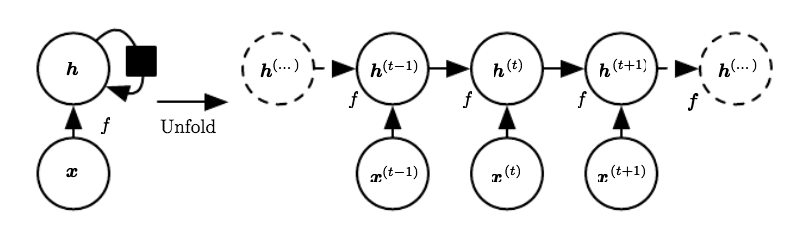
\includegraphics[width=0.9\columnwidth]{rnn.png}
\caption{Grafo de Computação de uma RNN genérica \citep{dlbook}}
\label{fig:rnngraph}
\end{figure}
%%%

Como podemos ver na Figura~\ref{fig:rnngraph}, a entrada $x$, ao lado do estado
interno $h$, são usados para calcular um novo estado. Nota-se que o vetor $h$,
bem como os parâmetros internos da RNN, são divididos entre iterações temporais.
\\

Essa classe de modelos normalmente é usada para modelagem de linguagem. Buscando
estimar uma distribuição de probabilidade $p(w_t | w_{t-1},w_{t-2},w_{t-3} \dots
) $ onde os $w_i$ são palavras subsequentes de um texto. Normalmente um modelo
dessa natureza busca resolver um problema de classificação, onde a próxima palavra
a ser prevista pelo modelo é uma entre todas as possibilidades de um certo
vocabulário. No caso do domínio em questão desejamos resolver um problema de
regressão, onde nosso alvo é um valor numérico. Para treinar um desses modelos,
precisamos usar como entrada exemplos subsequentes de dados, onde cada exemplo
de entrada tem um exemplo pareado de saída. Basicamente redes neurais
recorrentes funcionam recebendo um exemplo de entrada, criando uma representação
interna com o mesmo e então gerando uma saída e comparando essa saída com o
exemplo de saída real, gerando um erro. Finalmente, esse erro é propagado para
alterar seus parâmetros (com o fim de achar um conjunto de parâmetros que gere
boas previsões). \\ 


Como já explicado anteriormente, nossos dados de entrada e saída não estão necessariamente pareados perfeitamente dia a dia. Portanto, foi necessário achar intervalos de tempo nos dados onde existe esse pareamento. Isso reduz drasticamente quais períodos representados nos dados realmente podem ser usados para treinar um desses modelos.


\subsubsection{LSTM}
\label{sec:lstm}

LSTMs \citep{lstm} são um tipo de RNN que por meio de sua arquitetura permitem que sequências
maiores sejam processadas sem que o fluxo dos gradientes propagados pela rede se torne
numericamente problemático (i.e. tendendo a 0 ou a infinito). A
Figura~\ref{fig:lstm} ilustra o fluxo dos sinais em uma LSTM. Observa-se que a
entrada $x_t$ e o antigo estado $h_{t-1}$ são usados para o cálculo de diversos \textit{gates} ou \say{portas}, e
finalmente um novo estado $h_t$ é gerado.\\

\begin{figure}
\centering
\caption{Diagrama da arquitetura de uma LSTM}


\begin{tikzpicture}[
    prod/.style={circle, draw, inner sep=0pt},
    ct/.style={circle, draw, inner sep=5pt, ultra thick, minimum width=10mm},
    ft/.style={circle, draw, minimum width=8mm, inner sep=1pt},
    filter/.style={circle, draw, minimum width=7mm, inner sep=1pt, path picture={\draw[thick, rounded corners] (path picture bounding box.center)--++(65:2mm)--++(0:1mm);
    \draw[thick, rounded corners] (path picture bounding box.center)--++(245:2mm)--++(180:1mm);}},
    mylabel/.style={font=\scriptsize\sffamily},
    >=LaTeX
    ]

\node[ct, label={[mylabel]Cell}] (ct) {$c_t$};
\node[filter, right=of ct] (int1) {};
\node[prod, right=of int1] (x1) {$\times$}; 
\node[right=of x1] (ht) {$h_t$};
\node[prod, left=of ct] (x2) {$\times$}; 
\node[filter, left=of x2] (int2) {};
\node[prod, below=5mm of ct] (x3) {$\times$}; 
\node[ft, below=5mm of x3, label={[mylabel]right:Forget Gate}] (ft) {$f_t$};
\node[ft, above=of x2, label={[mylabel]left:Input Gate}] (it) {$i_t$};
\node[ft, above=of x1, label={[mylabel]left:Output Gate}] (ot) {$o_t$};

\foreach \i/\j in {int2/x2, x2/ct, ct/int1, int1/x1,
            x1/ht, it/x2, ct/it, ct/ot, ot/x1, ft/x3}
    \draw[->] (\i)--(\j);

\draw[->] (ct) to[bend right=45] (ft);

\draw[->] (ct) to[bend right=30] (x3);
\draw[->] (x3) to[bend right=30] (ct);

\node[fit=(int2) (it) (ot) (ft), draw, inner sep=0pt] (fit) {};

\draw[<-] (fit.west|-int2) coordinate (aux)--++(180:7mm) node[left]{$x_t$};
\draw[<-] ([yshift=1mm]aux)--++(135:7mm);
\draw[<-] ([yshift=-1mm]aux)--++(-135:7mm);

\draw[<-] (fit.north-|it) coordinate (aux)--++(90:7mm) node[above]{$x_t$};
\draw[<-] ([xshift=1mm]aux)--++(45:7mm);
\draw[<-] ([xshift=-1mm]aux)--++(135:7mm);

\draw[<-] (fit.north-|ot) coordinate (aux)--++(90:7mm) node[above]{$x_t$};
\draw[<-] ([xshift=1mm]aux)--++(45:7mm);
\draw[<-] ([xshift=-1mm]aux)--++(135:7mm);

\draw[<-] (fit.south-|ft) coordinate (aux)--++(-90:7mm) node[below]{$x_t$};
\draw[<-] ([xshift=1mm]aux)--++(-45:7mm);
\draw[<-] ([xshift=-1mm]aux)--++(-135:7mm);
\end{tikzpicture}


%%% Local Variables:
%%% mode: latex
%%% TeX-master: '../quali'
%%% End:

\label{fig:lstm}
\end{figure}




Uma rede LSTM possui três \say{portas}. Cada porta possui duas matrizes $W,U$ e um
vetor $b$ de parâmetros. Uma iteração da LSTM começa com o cálculo dos sinais
$o_t,i_t,f_t$.\\

\[f_t = \sigma_g(W_fx_t + U_fh_{t-1} + b_f)\]
\[i_t = \sigma_g(W_ix_t + U_ih_{t-1} + b_i)\]
\[o_t = \sigma_g(W_ox_t + U_oh_{t-1} + b_o)\]

O diferencial de uma LSTM é a propagação do sinal $c_t$, a célula de memória.
Esse valor depende de $f_t$ e $i_t$, que influenciam em como o valor da
célula de memória será atualizado na presente iteração. A equação a seguir
mostra como o valor da célula de memória é calculado. Onde $\circ$ é o produto Hadamard, ou apenas multiplicação entrada por entrada de
duas matrizes ou vetores. \\

\[c_t = f_t \circ c_{t-1} + i_t \circ \sigma_c(W_cx_t + U_ch_{t-1} + b_c)\]

Nota-se que $f_t$
define quanto do valor antigo da célula de memória deve participar no cálculo do
seu novo valor. 
Da mesma maneira $i_t$ define quanto da nova entrada deve ser usada no cálculo desse valor.
Em outras palavras, as portas $i_t$ e $f_t$ definem o quanto a LSTM deve,
respectivamente, \say{lembrar} e \say{esquecer}.


O novo estado da LSTM é então calculado por: \\
\[h_t = o_t \circ \sigma_h(c_t)\]




\subsubsection{Rede Encoder-Decoder}
\label{sec:encdec}
Redes Encoder-Decoder são usadas para modelagem de sequência para
sequência, ou seja, para receber dados sequenciais como entrada e gerar
sequências como saída \citep{dlbook}. Esses modelos possuem duas partes, ambas compostas por
RNNs. \\

\begin{figure}[H]
\centering
\begin{tikzpicture}[font=\sffamily]
\node[fill=brown!90!black, text=white, font=\sffamily\small, inner sep=2pt] (a) {\begin{tabular}{@{}r@{}}-0.2\\-0.1\\0.1\\0.4\\-0.3\\1.1\end{tabular}};

\node[fit=(a.north) (a.south), inner sep=1pt, right=1mm of a, minimum width=2cm, label=center:Decoder] (dec) {};
\node[fit=(a.north) (a.south), inner sep=1pt, left=1mm of a, minimum width=2cm, label=center:Encoder] (enc) {};

\begin{scope}[on background layer]
\fill[cyan!30] (dec.north west)--([yshift=5mm]dec.north east)--([yshift=-5mm]dec.south east)--(dec.south west)--cycle;
\fill[cyan!30] (enc.north east)--([yshift=5mm]enc.north west)--([yshift=-5mm]enc.south west)--(enc.south east)--cycle;
\end{scope}

\node[right=1mm of dec, fill=blue, single arrow] (b) {\phantom{a}};
\node[align=left, right=1mm of b] {Sequência de\\ saída};

\node[left=1mm of enc, fill=blue, single arrow] (c) {\phantom{a}};
\node[align=left, left=1mm of c] {Sequência de\\ entrada};
\end{tikzpicture}
%%% Local Variables:
%%% mode: latex
%%% TeX-master: t
%%% End:

\caption{ Diagrama de Rede Encoder-Decoder.\\ Modificado de \citep{encdec}}

\end{figure}
  
O \textbf{encoder} é uma RNN que busca receber uma sequência de entrada de
tamanho arbitrário e gerar uma representação como saída, o seu estado interno,
representando em marrom no diagrama acima. O \textbf{Decoder} então recebe essa representação interna (também chamada
de \textit{codificação}) e usa-a para gerar saídas sequencialmente, podendo
então gerar essas sequências de duas formas: O Decoder pode usar as suas próprias saídas
como entrada para gerar a saída da próxima iteração temporal, ou então usar dados de treinamento como
entradas, essa última forma chamada de \textit{teacher forcing}. No diagrama
está indicado o acoplamento entre o decoder e o encoder. Essa codificação é apenas
um vetor (cuja dimensão é um \textit{hiper-parâmetro} de treinamento) que resume a
informação sequencial lida pelo encoder e a transmite para o decoder.
Hiper-parâmetros são parâmetros do problema de aprendizado que são definidos
pelo programador e não fazem parte dos valores aprendidos pelo algoritmo de
aprendizado. É comum que se realizem diversos experimentos com diferentes
valores de hiper-parâmetros e se escolha os que geraram melhores resultados. 
\\

Redes encoder-decoder são muito usadas para aprender \textit{representações} para os
dados. Isso quer dizer que as codificações da rede encoder-decoder são frutos de
transformações no espaço das entradas que buscam extrair a informação mais útil
para o objetivo do aprendizado. Podemos pensar nessas transformações como
mudanças de coordenadas nas quais estamos representando os dados. Justamente o problema de aprender
representações estimulou desde 2006 uma redescoberta do DL \citep{dlbook}. Criar
operações que transformem os dados de entrada de modo a facilitar o aprendizado
pode levar anos se essa tarefa for colocada na mão de especialistas humanos
\citep{dlbook}, então é uma capacidade valiosa proporcionada por algoritmos de
DL como redes encoder-decoder. \\



\section{Modelos Bayesianos}

Apesar de se tratarem de aproximações de verdadeiras inferências bayesianas, os
modelos nessa seção buscam unir a acurácia de métodos frequentistas de ML com a
margem de incerteza proveniente do uso da Lei de Bayes.

\subsection{Inferência Bayesiana em Machine Learning}
\label{sec:bayesinf}
O tratamento Bayesiano para modelos de ML é bastante diverso dos frequentistas \citep{dlbook}.
Em uma análise frequentista estima-se um valor de $\theta$ e então todas as
predições são feitas a partir desse valor. No caso Bayesiano se consideram todos
os possíveis valores de $\theta$ ao se fazer uma predição. É preciso especificar
a incerteza \textbf{a priori} $p(\theta)$ sobre os parâmetros, e então
consideramos que os dados \textbf{foram observados} e usa-se a lei de Bayes para
calcular a \textbf{probabilidade} posterior $p(\theta | X,Y)$ usando para tal
$p(Y |X, \theta)$, a chamada verossimilhança \citep{bayesml}. 

\[    p(\theta | X,Y) = \frac{p(Y| X,\theta) p(\theta)}{p(Y)}   \]

Finalmente, para realizar uma inferência devemos integrar por toda a distribuição $p(\theta)$ marginalizando esse parâmetro. Se por exemplo queremos uma nova anotação $y^*$ para um novo dado $x^*$:


\begin{equation}
  \label{eq:int}
p(y^* | x^* , X,Y) = \int  p(y^* | x^*,\theta) p(\theta | X,Y)  d\theta 
\end{equation}

Essa integral é geralmente intratável pela dificuldade de se calcular
analiticamente $p(\theta | X,Y)$ \citep{ubertime}, devemos então tentar aproximar essa distribuição
pela chamada distribuição variacional, $q^*(\theta)$, e então a solução numérica da integral, com uma boa escolha de $q^{*}$, se torna uma aproximação $q^{*}(y^{*}| x^{*})$: 

\begin{align*}
  \label {eq:pq}
    p(y^* | x^* , X,Y) &\approx \int  p(y^* | x^*,W) q^*(W)dW \\
                       &= q^*(y^* | x^*)
\end{align*}

Esse processo chama-se Inferência Variacional e seu objetivo ( i.e. aproximar a distribuição variacional da distribuição real $p(\theta | X,Y)$)
é alcançado minimizando-se a seguinte inequação, o \textit{Variational Lower Bound} \citep{bayesml}: \\

\begin{equation}
  \label {eq:ine}
  \mathcal{L}_{VI} = \int q(W) \log p(Y | X,W)dW - \mathnormal{KL}(q(W) ||p(W)) \\
                  \leq \log p(Y|X) 
\end{equation}



\subsubsection{Rede Neural Bayesiana}

Redes Neurais Bayesianas, como qualquer modelo bayesiano, especificam uma distribuição \textit{a priori} da matriz $W$ de parâmetros.
A Lei de Bayes é então aplicada para se calcular a distribuição posterior de $W$, ao invés de uma estimativa pontual, como usualmente é feito no tratamento frequentista.
Devido a complexidade desses modelos, é intratável calcular analiticamente essa distribuição posterior, então diversos métodos foram propostos para uma aproximação \cite{Gal2016Uncertainty}.
O Método aplicado nesse trabalho é o Monte Carlo Dropout, que não requer nenhuma mudança na arquitetura do modelo para realizar a inferência. Consistindo apenas de uma reinterpretação de uma Rede Neural implementada com uma técnica de regularização chamada Dropout. 

\subsubsection{Monte Carlo Dropout}

O processo de Inferência Variacional pode ser aproximado em uma rede neural pela técnica do Monte Carlo Dropout \citep{dropbayes}. \\

O Monte Carlo Dropout consiste no uso de \textbf{Dropout} em todas as camadas da rede
neural, i.e. descartar ativações aleatoriamente entre duas camadas da rede com
probabilidade $p$.\\

\begin{figure}
  \centering
  \resizebox {\columnwidth} {!} {



\begin{tikzpicture}

	\node[circle, draw, thick] (i1) {};
	\node[circle, draw, thick, above=2em of i1] (i2) {};
	\node[circle, draw, thick, above=2em of i2] (i3) {};
	\node[circle, draw, thick, below=2em of i1] (i4) {};
	\node[circle, draw, thick, below=2em of i4] (i5) {};
	
	\node[circle, draw, thick, right=4em of i1] (h1) {};
	\node[circle, draw, thick, right=4em of i2] (h2) {};
	\node[circle, draw, thick, right=4em of i3] (h3) {};
	\node[circle, draw, thick, right=4em of i4] (h4) {};
	\node[circle, draw, thick, right=4em of i5] (h5) {};
	
	\node[circle, draw, thick, right=4em of h1] (hh1) {};
	\node[circle, draw, thick, right=4em of h2] (hh2) {};
	\node[circle, draw, thick, right=4em of h3] (hh3) {};
	\node[circle, draw, thick, right=4em of h4] (hh4) {};
	\node[circle, draw, thick, right=4em of h5] (hh5) {};
	
	\node[circle, draw, thick, right=4em of hh2] (o1) {};
	\node[circle, draw, thick, right=4em of hh4] (o2) {};
	
	\draw[-stealth, thick] (i1) -- (h1);
	\draw[-stealth, thick] (i1) -- (h2);
	\draw[-stealth, thick] (i1) -- (h3);
	\draw[-stealth, thick] (i1) -- (h4);
	\draw[-stealth, thick] (i1) -- (h5);
	\draw[-stealth, thick] (i2) -- (h1);
	\draw[-stealth, thick] (i2) -- (h2);
	\draw[-stealth, thick] (i2) -- (h3);
	\draw[-stealth, thick] (i2) -- (h4);
	\draw[-stealth, thick] (i2) -- (h5);
	\draw[-stealth, thick] (i3) -- (h1);
	\draw[-stealth, thick] (i3) -- (h2);
	\draw[-stealth, thick] (i3) -- (h3);
	\draw[-stealth, thick] (i3) -- (h4);
	\draw[-stealth, thick] (i3) -- (h5);
	\draw[-stealth, thick] (i4) -- (h1);
	\draw[-stealth, thick] (i4) -- (h2);
	\draw[-stealth, thick] (i4) -- (h3);
	\draw[-stealth, thick] (i4) -- (h4);
	\draw[-stealth, thick] (i4) -- (h5);
	\draw[-stealth, thick] (i5) -- (h1);
	\draw[-stealth, thick] (i5) -- (h2);
	\draw[-stealth, thick] (i5) -- (h3);
	\draw[-stealth, thick] (i5) -- (h4);
	\draw[-stealth, thick] (i5) -- (h5);
	
	\draw[-stealth, thick] (h1) -- (hh1);
	\draw[-stealth, thick] (h1) -- (hh2);
	\draw[-stealth, thick] (h1) -- (hh3);
	\draw[-stealth, thick] (h1) -- (hh4);
	\draw[-stealth, thick] (h1) -- (hh5);
	\draw[-stealth, thick] (h2) -- (hh1);
	\draw[-stealth, thick] (h2) -- (hh2);
	\draw[-stealth, thick] (h2) -- (hh3);
	\draw[-stealth, thick] (h2) -- (hh4);
	\draw[-stealth, thick] (h2) -- (hh5);
	\draw[-stealth, thick] (h3) -- (hh1);
	\draw[-stealth, thick] (h3) -- (hh2);
	\draw[-stealth, thick] (h3) -- (hh3);
	\draw[-stealth, thick] (h3) -- (hh4);
	\draw[-stealth, thick] (h3) -- (hh5);
	\draw[-stealth, thick] (h4) -- (hh1);
	\draw[-stealth, thick] (h4) -- (hh2);
	\draw[-stealth, thick] (h4) -- (hh3);
	\draw[-stealth, thick] (h4) -- (hh4);
	\draw[-stealth, thick] (h4) -- (hh5);
	\draw[-stealth, thick] (h5) -- (hh1);
	\draw[-stealth, thick] (h5) -- (hh2);
	\draw[-stealth, thick] (h5) -- (hh3);
	\draw[-stealth, thick] (h5) -- (hh4);
	\draw[-stealth, thick] (h5) -- (hh5);
	
	
	\draw[-stealth, thick] (hh1) -- (o1);
	\draw[-stealth, thick] (hh1) -- (o2);
	\draw[-stealth, thick] (hh2) -- (o1);
	\draw[-stealth, thick] (hh2) -- (o2);
	\draw[-stealth, thick] (hh3) -- (o1);
	\draw[-stealth, thick] (hh3) -- (o2);
	\draw[-stealth, thick] (hh4) -- (o1);
	\draw[-stealth, thick] (hh4) -- (o2);
	\draw[-stealth, thick] (hh5) -- (o1);
	\draw[-stealth, thick] (hh5) -- (o2);
	
	\draw[-stealth, double, dashed, thick] (5.5,0) -- node[above] {dropout} (8.6, 0);
	
	
	%%% BOUNDARY %%%
	
	\node[circle, draw, thick, red, fill=red!10, right=15em of hh1] (i1) {};
	\node[circle, draw, thick, red, fill=red!10, above=2em of i1] (i2) {};
	\node[circle, draw, thick, above=2em of i2] (i3) {};
	\node[circle, draw, thick, below=2em of i1] (i4) {};
	\node[circle, draw, thick, below=2em of i4] (i5) {};
	
	\node[red] (icr) at (i1) {$\mathlarger{\mathlarger{\mathlarger{\mathlarger{\mathlarger{\bm{\times}}}}}}$};
	\node[red] (icr) at (i2) {$\mathlarger{\mathlarger{\mathlarger{\mathlarger{\mathlarger{\bm{\times}}}}}}$};
	
	\node[circle, draw, thick, red, fill=red!10, right=4em of i1] (h1) {};
	\node[circle, draw, thick, right=4em of i2] (h2) {};
	\node[circle, draw, thick, red, fill=red!10, right=4em of i3] (h3) {};
	\node[circle, draw, thick, red, fill=red!10, right=4em of i4] (h4) {};
	\node[circle, draw, thick, right=4em of i5] (h5) {};
	
	\node[red] (icr) at (h1) {$\mathlarger{\mathlarger{\mathlarger{\mathlarger{\mathlarger{\bm{\times}}}}}}$};
	\node[red] (icr) at (h3) {$\mathlarger{\mathlarger{\mathlarger{\mathlarger{\mathlarger{\bm{\times}}}}}}$};
	\node[red] (icr) at (h4) {$\mathlarger{\mathlarger{\mathlarger{\mathlarger{\mathlarger{\bm{\times}}}}}}$};
	
	\node[circle, draw, thick, right=4em of h1] (hh1) {};
	\node[circle, draw, thick, red, fill=red!10, right=4em of h2] (hh2) {};
	\node[circle, draw, thick, right=4em of h3] (hh3) {};
	\node[circle, draw, thick, red, fill=red!10, right=4em of h4] (hh4) {};
	\node[circle, draw, thick, right=4em of h5] (hh5) {};
	
	\node[red] (icr) at (hh2) {$\mathlarger{\mathlarger{\mathlarger{\mathlarger{\mathlarger{\bm{\times}}}}}}$};
	\node[red] (icr) at (hh4) {$\mathlarger{\mathlarger{\mathlarger{\mathlarger{\mathlarger{\bm{\times}}}}}}$};
	
	\node[circle, draw, thick, right=4em of hh2] (o1) {};
	\node[circle, draw, thick, right=4em of hh4] (o2) {};
	
	\draw[-stealth, thick] (i3) -- (h2);
	\draw[-stealth, thick] (i3) -- (h5);
	\draw[-stealth, thick] (i4) -- (h2);
	\draw[-stealth, thick] (i4) -- (h5);
	\draw[-stealth, thick] (i5) -- (h2);
	\draw[-stealth, thick] (i5) -- (h5);
	
	\draw[-stealth, thick] (h2) -- (hh1);
	\draw[-stealth, thick] (h2) -- (hh3);
	\draw[-stealth, thick] (h2) -- (hh5);
	\draw[-stealth, thick] (h5) -- (hh1);
	\draw[-stealth, thick] (h5) -- (hh3);
	\draw[-stealth, thick] (h5) -- (hh5);
	
	\draw[-stealth, thick] (hh1) -- (o1);
	\draw[-stealth, thick] (hh1) -- (o2);
	\draw[-stealth, thick] (hh3) -- (o1);
	\draw[-stealth, thick] (hh3) -- (o2);
	\draw[-stealth, thick] (hh5) -- (o1);
	\draw[-stealth, thick] (hh5) -- (o2);

\end{tikzpicture}


%%% Local Variables:
%%% mode: latex
%%% TeX-master: t
%%% End:
}
  \label{fig:dropout}
  \caption{Representacão do uso de Dropout em uma rede neural}
\end{figure}

Formalmente, para um vetor de ativações $a$ na saída de uma
camada da rede neural, amostramos um vetor de \textit{máscara} $\epsilon$ de uma
distribuição de Bernoulli cujo parâmetro é $p$, i.e. $\epsilon \sim Bernoulli(p)$.
Finalmente, o novo vetor de ativações é calculado por $\epsilon * a$. O efeito desse
processo é de zerar aleatoriamente entradas do vetor de ativação.
\\

Seja uma rede neural com apenas uma camada, cujos parâmetros são $W$ e $b$, como explicado na Sessão~\ref{sec:nn}. Amostrar uma máscara para o vetor de ativação a cada computação da rede é equivalente a considerar que estamos amostrando os próprios pesos da rede a cada computação \citep{dropbayes}. Seja $W$ a matriz de pesos da rede neural, então, escrevemos que a cada computação essa matriz é calculada amostrando-se um vetor $\epsilon$ e multiplicando pelo valor atual dos pesos: \\

\newcommand{\diag}{\mathop{\mathrm{diag}}}

$$    W^*   \sim \mathnormal{q}(W) $$
$$    W^*  = \diag(\epsilon) * W $$


A função de custo de uma rede neural com dropout em todas as camadas pode ser escrita da seguinte forma:

\[     \mathcal{L}_{dropout} = \sum^N_{N=1} (y_n - \mathnormal{f}^{W^*,b}(x_n))^2 + \boldsymbol{\alpha}\{W^2,b^2\} \]


\citep{dropbayes} demonstram que a aplicação do dropout em todas as camadas da rede faz com que a minimização
do objetivo de treinamento seja equivalente a minimização da Inequação~\ref{eq:ine}, i.e. o objetivo da Inferência Variacional.\\

Então, após realizado o treinamento, a saída do nosso modelo é uma amostragem da distribuição $q(y^* | x^* , \theta)$.
A média e variância amostrais de um conjunto de diversas realizações estocásticas da saída da rede são estimadores não-enviesados das médias e variâncias reais:

\begin{align*}
  \label{eq:aproxs}
  \widetilde{\mathbb{E}}[y^*] &=
   \frac{1}{B}\sum^B_{B=1}\mathnormal{f}^{\hat{W},b}(x^*) = \frac{1}{B}\sum^B_{B=1}\hat{y}^*_{(B)}\\ 
   \widetilde{\mathit{Var}}[y^*]  &= \frac{1}{B}\sum^B_{B=1}(\hat{y}^*_{(B)} - \bar{y}^*)^2 
 \end{align*}

\subsubsection{Modelo Encoder-Decoder-Forecaster}

Iremos reproduzir nesse trabalho o modelo proposto em \citep{ubertime}. A
arquitetura consiste em uma rede \textbf{encoder-decoder} que aprende codificações da
série temporal (i.e. uma representação que extraia informações úteis para o
problema) e então uma rede \textbf{forecaster} que usa essas codificações ao lado de
variáveis exógenas a série temporal para realizar predições.  


\begin{figure}[H]
\centering
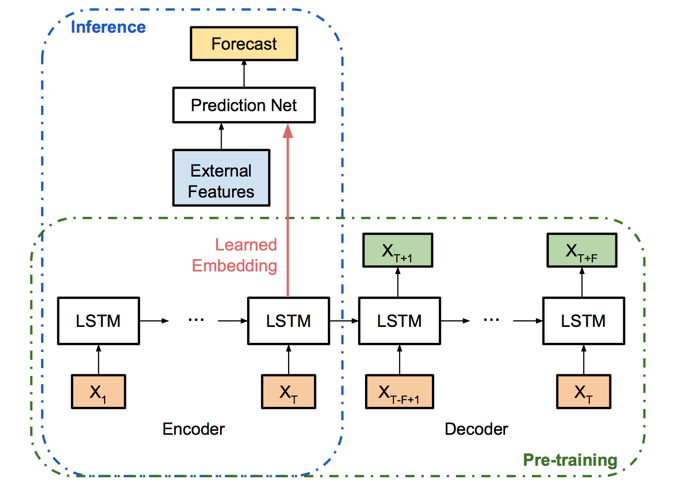
\includegraphics[width=0.9\columnwidth]{uber.png}
\caption{Arquitetura do modelo proposto por \citep{ubertime}}
\end{figure}


Durante o pré-treinamento a rede encoder-decoder consome sequências de $F + T$ dias
da série temporal. O encoder cria uma representação vetorial $h$ depois de
receber como entrada os primeiros $T$ dias da sequência. Então, $h$ é usado como
inicialização do estado interno do decoder, e esse então consume mais $F$
entradas da sequência. Para o decoder, se em uma iteração sua entrada é $X_i$,
então sua saída será comparada com $X_{i+1}$, e esse erro é propagado após lidas
todas as entradas para que a representação $h$ proveniente do encoder possa se
tornar mais informativa.


Esse modelo também possui outra característica importante. Todas as camadas da
redes neurais que compõe o encoder, o decoder e o forecaster possuem
Dropout com probabilidade $p$. Ou seja, podemos usar a técnica do Monte
Carlo Dropout para estimar a variância de cada predição feita por esse modelo. A
rede então se torna um modelo bastante robusto para consumir séries temporais,
assim realizando predições e incertezas.\\


Essa capacidade do modelo o torna mais interessante do que meramente usar uma
rede LSTM para o problema de regressão. Agora iremos definir como a informação
de incerteza pode ser calculada usando esse modelo. \\

Na seção~\ref{sec:reglog} definimos um problema de regressão linear sob o ponto
de vista Bayesiano. Para esse problema assumimos a verossimilhança como $p(y |f^W(x))$.
Onde $f^W(.)$ é a rede Encoder-Forecaster após o treino.
Como estamos lidando com regressão, podemos especificar ainda essa distribuição
como \citep{ubertime}:  

\begin{equation}
  \label{eq:reg}
 y| W \sim \mathcal{N}(y;f^W(x),\,\sigma^2)
\end{equation}

 Na seção~\ref{sec:bayesinf} explicamos como na Inferência Bayesiana para marginalizamos os parâmetros $W$ e calculamos a distribuição $p(y^*
 | x^*)$ pela Integral~\ref{eq:int}, o que é intratável para esse modelo sem uma aproximação.
 A variância de $p(y^{*} | x^{*})$ quantifica a incerteza das predições
 \citep{dropbayes}, e pode ser decomposta usando a lei da variância total \citep{ubertime}, e parte dessa soma pode ser estimada pela técnica do MC Dropout: \\



\[ Var(y^* | x^*) = Var[\mathop{\mathbb{E}}(y^* | W,x^*)] +
  \mathop{\mathbb{E}}[Var(y^* | W,x^*)] \]

Como o primeiro termo dessa soma dentro do operador do valor esperado segue uma distribuição normal
(Equação~\ref{eq:reg}), podemos substituí-lo pela sua média. O
segundo termo será definido como $\sigma^2$: \\ 
 
\[ Var(y^* | x^*) = Var(f^W(x^*)) + \sigma^2 \] 


Vemos que nossa incerteza é decomposta em dois termos. $Var(f^W(x^*))$ denota a
nossa ignorância em relação aos parâmetros do modelo, referida como
\textit{incerteza do modelo}. $\sigma^2$ seria então o \textit{ruído inerente} ao
processo gerador de dados.
 
A estimativa de $Var(f^W(x^*))$ se dá pela técnica do MC Dropout. A variância
será aproximada pela variância amostral de $B$ predições estocásticas calculadas
na rede com camadas de Dropout ativadas. Seja $\{\hat{y}^*_{(1)},\hat{y}^*_{(2)}, \dots
\hat{y}^*_{(B)}\}$ o vetor de predições amostrado dessa forma, e $\hat{y}^*$ sua
média amostral, temos: \\

\[   Var(f^W(x^*))  = \frac{1}{B}\sum^B_{B=1}(\hat{y}^*_{(B)} - \hat{y}^*)^2  \]


O ruído inerente das medidas é estimado usando os \textit{dados de validação},
i.e. aqueles não
usados durante o treinamento. Como
proposto por \citep{ubertime}, sejam $(X',Y')$ nossos dados de validação, com
$V$ entradas. Esses dados são independentes do nosso modelo
treinado $f^W(.)$, então podemos usa-los para estimar o ruído inerente do
modelo: \\

\[ \hat{\sigma}^2 = \frac{1}{V}\sum^V_{V=1}(y'_v - f^W(x'_v))^2 \]

Finalmente, sejam nossa incerteza do modelo $\eta_1^2$ e o ruído inerente
$\eta^2_2$, calcula-se a incerteza total do modelo por: \\

\[  \eta_{tot} = \sqrt{  \eta_1^2 + \eta_2^2 }  \]


\subsection{Modelo DeepAR}

O modelo \textit{DeepAR}, proposto em \citep{deepar}, é baseado em redes neurais recorrentes auto-regressivas,
i.e. que tem sua saída realimentada na entrada da iteração posterior. Por meio da função de verossimilhança binomial esse modelo é capaz
de realizar predições probabilísticas.

O modelo é descrito pela seguinte equação, onde $h$ é uma RNN implementada com células de LSTMs:

\[
h_{i,t} = h(h_{i,t-1},y^*_{i,t-1},x_{i,t}, \theta)
\]

Nota-se que o estado da RNN tem como argumento o estado anterior e os parâmetros de entrada, mas também a saída da iteração passada do modelo, $y^*_{i,t-1}$. \\

A verossimilhança do modelo, $\mathcal{L}(y_{i,t} | \omega(h_{i,t}))$, é uma distribuição fixa cujos parâmetros são dados por uma função $\omega$ da saída $h$ do modelo. Usaremos uma função de verossimilhança binomial já que estamos otimizando um objetivo de regressão, assim como na Equação~\ref{eq:logver}:

\[
\mathcal{L}(y | \mu,\sigma) = {(2\pi\sigma^2)}^{-\frac{1}{2}} \exp(-  \frac{-y - \mu^2}{2\sigma^2})  
\]

A média $\mu$ e o desvio-padrão $\sigma$ são calculados diretamente pela saída do modelo. Para a média, usamos uma transformação linear parametrizada por $W_{\mu},b_{\mu}$. No caso do desvio-padrão, para garantirmos que ele seja maior que 0, usamos uma função \textit{softplus} após uma transformação linear análoga ao caso da média, parametrizada por  $W_{\sigma},b_{\sigma}$.\\

\[ \mu(h_{i,t}) = W_{\mu}h_{i,t} + b_{\mu} \]

\[ \sigma(h_{i,t}) = \log(1 + \exp(W_{\sigma}h_{i,t}+ b_{\sigma})) \]


\subsubsection{Treinamento}



O modelo possui uma etapa de treinamento e uma etapa de validação. O Diagrama~\ref{dig:dar} ilustra como o modelo se comporta em cada um desses momentos: \\


TO-DO-IMAGEM \\


O funcionamento do modelo é similar ao de uma rede Encoder-Decoder, como visto na Sessão~\ref{sec:encdec}, o modelo deve consumir intervalos de $F$ valores dos parâmetros da série temporal, essa seria a fase do \textit{encoding}, para então gerar $T$ anotações dos dados na fase do \textit{decoding}. Durante o treinamento o erro do modelo é calculado comparando-se uma anotação gerada durante a fase de encoding $y^{*}_{t}$ com o seu valor real $y_{t}$. \\

Durante o \textbf{treinamento} o modelo recebe como entrada do instante $t$, o valor real da série no instante $t-1$. \\
  
Durante a \textbf{validação} o modelo é \textbf{realimentado} com a anotação $y^{*}_{t-1}$ gerada na iteração anterior. \\ 



O treinamento do modelo é feito pela maximização da log-verossimilhança: \\

\[
\theta = argmax \sum_i{\log(\mathcal{L}(y_i | \omega(h_{i})))}
\]


Uma saída $y^*_{i,t}$ do modelo é calculada por meio de uma amostragem da Gaussiana determinada pela média e variância calculadas: \\

\[
 y^*_{i,t} \sim \mathcal{N}(\mu,\sigma) 
\]

\subsection{Modelo com Deep Factors}

O modelo \textit{Deep Factors with Gaussian Process} \citep{deepfactors} separa o problema de predição em uma parte \textbf{local}, modelada por um Processo Gaussiano que gera incertezas, e uma parte \textbf{fixa}, modelada por uma rede neural recorrente treinada em diversas séries temporais do mesmo domínio.


Um Processo Gaussiano é uma coleção de variáveis aleatórias,
sendo que qualquer subconjunto finito das mesmas é descrito por uma Distribuição Gaussiana conjunta \citep{gpml}. \\

Um Processo Gaussiano é descrito completamente pela sua função de média e sua função de covariância. Usamos essas duas funções para amostrar o processo estocástico $f(x)$ que está sendo modelado: \\

\[
f(x) \sim \mathcal{GP}( m(x), K(x,x'))
\]

É comum que se escolha como função média apenas a constante 0 \citep{gpml}.  A função de covariância, as vezes chamada de Kernel, deve especificar a covariância entre os pares de variáveis aleatórias (i.e. os dados), para problemas de regressão é usual escolhermos um Kernel que relacione uma medida de distância das variáveis de entrada. Como por exemplo o \textit{quadrado da função exponencial}: \\

\[
  K(x,x') = \exp(-\frac{1}{2}\abs{x - x'}^2)
\]


\subsubsection{Modelo Generativo}

O modelo Deep Factors então é composto por duas partes, a combinação linear de ambas é a saída do modelo i.e. a emissão de valores de saída amostrados: \\


\[
    \textbf{Gerador de ruído local: }  r_i \sim \mathcal{GP} (0, K_i(.,.))
\]

O ruído é gerado por um Processo Gaussiano com média 0 e função de covariância exponencial. O Processo calcula incertezas em todos os pontos $x_{i,t}$ da série temporal $i$.
  
\[
  \textbf{Gerador da parte fixa aprendida globalmente: }  f_{i,t} = W_ig_t(x_{i,t})
\]
A função $g_t$ é uma RNN, no caso desse trabalho uma célula LSTM, que recebe como entrada um certo número $T$ de passos da série temporal, e então emite como saída um horizonte finito $F$ de predições.
\[
  \textbf{Emissão: }  y^*_{i,t} \sim p(. | u_{i,t}) , u_{i,t} = r_{i,t} + f_{i,t}  
\]

\subsubsection{Treinamento}

Como $p(. | u_{i,t})$ é distribuida normalmente, não precisamos de inferência para calcular a verossimilhança marginal do modelo, que é dada por: \\

\[
p(y_{i}) = \mathcal{N}(f_i,K_i + \sigma_i^2\mathcal{I})
\]

O objetivo de treinamento é achar o conjunto de parâmetros da RNN e do Processo Gaussiano que minimizem a log-verossimilhança conjunta dos dados: \\
\[
\theta = argmax \sum_i{\log(p(y_i))}
\]


%%% Local Variables:
%%% mode: latex
%%% TeX-master: "../quali"
%%% TeX-command-default: "latexmk"
%%% bibtex-file-path: "../bibliografia"
%%% End: